% 4 paragraph intro
To communicate successfully, speakers and listeners must share a common system of semantic meaning in the language they are using. 
These meanings are \emph{social conventions} in the sense that they are arbitrary to some degree, but sustained by stable expectations that each person holds about others in their community \cite{lewis_convention:_1969,bicchieri_grammar_2006, hawkins2019emergence}.
Importantly, these expectations extend to complete strangers.
An English speaker may order an ``espresso'' at any café in the United States and expect to receive (roughly) the same kind of drink.
At the same time, meaning can be remarkably flexible and \emph{partner-specific}.
The same words may be interpreted differently by different listeners, or take on new \emph{ad hoc} senses over the course of a conversation \cite{clark_using_1996}. 
Interactions between friends and colleagues are filled with proper names, technical jargon, slang, shorthand, and inside jokes, many of which are unintelligible to outside observers.

The tension between these two basic observations, global stability and local flexibility, has posed a challenging and persistent puzzle for theories of convention.
Many influential computational accounts explaining how stable social conventions emerge in populations  do not allow for partner-specific meaning at all \cite<e.g.>{hurford1989biological,shoham1997emergence,barr_establishing_2004,skyrms2010signals,steels2011modeling,young_evolution_2015}.
These accounts typically examine groups of interacting agents who update their representations of language after each interaction.
While the specific update rules range from simple associative mechanisms \cite<e.g.>{steels_self-organizing_1995} or heuristics \cite<e.g>{Young96_EconomicsOfConvention} to more sophisticated deep reinforcement learning algorithms \cite<e.g.>{tieleman2019shaping,graesser2019emergent,mordatch2017emergence}, all of these accounts assume that agents update a single, monolithic representation of language to be used with every partner, and that agents do not (knowingly) interact repeatedly with the same partner.

Conversely, accounts emphasizing rapid alignment \cite{pickering2004toward} or the development of partner-specific common ground \cite{ClarkMarshall1981,ClarkWilkesGibbs86_ReferringCollaborative} across extended interactions with the same partner typically do not specify mechanisms by which community-wide conventions arise over longer timescales.
The philosopher Donald Davidson articulated one of the most radical of these accounts.
According to \citeA{davidson1984communication,davidson_nice_1986,davidson1994social}, while we bring background expectations (``prior theories'') into interactions, it is the ability to coordinate on \emph{partner-specific} meanings (``passing theories'') that is ultimately responsible for communicative success: 
\begin{quote}
\footnotesize\emph{In order to judge how he will be interpreted, [the speaker] uses a picture of the interpreter’s readiness to interpret along certain lines, [...] the starting theory of interpretation. %Central to this picture is what the speaker believes is 
%The speaker does not necessarily speak in such a way as to prompt the interpreter to apply this prior theory; he may deliberately dispose the interpreter to modify his prior theory. But the speaker’s view of the interpreter’s prior theory is not irrelevant to what he says, nor to what he means by his words; it is an important part of what he has to go on if he wants to be understood.
As speaker and interpreter talk, their ``prior'' theories become more alike; so do their ``passing'' theories. 
The asymptote of agreement and understanding is when passing theories coincide. 
%But the passing theory cannot in general correspond to an interpreter’s linguistic competence. 
Not only does it have its changing list of proper names and gerrymandered vocabulary, but it includes every successful use of any other word or phrase, no matter how far out of the ordinary [...] 
%Every deviation from ordinary usage, as long as it is agreed on for the moment [...] is in the passing theory as a feature of what the words mean on that occasion. 
Such meanings, transient though they may be, are literal. \\\cite[p.~261]{davidson_nice_1986}.}
\end{quote}
This line of argument led \citeA{davidson_nice_1986} to conclude that ``there is no such thing as a language'' (p.~265), and to abandon appeals to convention altogether (see \citeNP{heck_idiolect,lepore2007reality,hacking1986nice,dummett1994} for further discussion of Davidson's view; \citeNP{armstrong2016coordination,armstrong2016problem}, provides a philosophical foundation for our synthesis).%\footnote{ In Davidson's terminology, the system of meanings given by from convention is called the agent's \emph{prior} theory, while the ad hoc systems they form with their partner on the fly are called their \emph{passing} theories. We maintain this distinction, but instead call these \emph{global} conventions and \emph{local} or \emph{ad hoc} conventions, respectively, to emphasize their commonality.}.

In this paper, we propose an account of coordination and convention that aims to reconcile the emergence of community-level conventions with partner-specific common ground in a unified cognitive model.
This theory is motivated by the computational problems facing individual agents who must communicate with one another in a variable and non-stationary world. 
We suggest that three core cognitive capacities are needed for an agent to solve this problem:
\begin{description}
\item[C1:] the ability to represent \textbf{variability} about what words will mean to different partners,
\item[C2:] the ability to coordinate on partner-specific meanings via flexible \textbf{online learning}, and
\item[C3:] the ability to gradually \emph{generalize} stable expectations about meaning from individual interactions.
\end{description}
These properties are naturally formalized in a hierarchical Bayesian framework, which we call CHAI (Continual Hierarchical Adaptation through Inference). 
Indeed, one of our central theoretical aims is to ground the problem of convention formation --- a fundamentally interactive, social phenomenon --- in the same domain-general cognitive mechanisms supporting learning in other domains where abstract, shared properties need to be inferred along with idiosyncratic particulars of instances \cite{berniker2008estimating,GoodmanUllmanTenenbaum11_TheoryOfCausality,tenenbaum_how_2011,kleinschmidt2015robust}.

%\begin{enumerate}
%\item \textbf{Lexical uncertainty:} When we first encounter a new communication partner in a new context, we call upon some representation about what we think different signals mean to them. This representation of meaning must be sensitive to the overall statistics of the population: more people are familiar with the use of \emph{dog} to refer to the beloved pet than \emph{sclerotic aorta} to refer to the potentially dangerous health condition. It must also be sensitive to the immediate context of the interaction: a cardiologist should have different expectations about a novel colleague than a novel patient.
%\item \textbf{Rapid adaptation:} Within a few minutes of conversation, we can considerably strengthen our expectations about our partner's lexicon based on earlier utterances and feedback, and adjust our own usage accordingly. For example, even if we are not initially familiar with the term \emph{sclerotic aorta}, a few minutes spent discussing the condition in simpler terms should make us more confident using the term with that partner in the future. This social learning mechanism must allow for signal \emph{reduction} -- simpler, more efficient ways of referring to the same thing over time -- and \emph{path-dependence}: early reinforcement of certain meanings increases their later usage, however arbitrary or provisional they began. 
%\item \textbf{Generalization:} When we encounter the same partner in a new context, we should expect some `stickiness' from previous learning. Language does not reset at context boundaries. In addition, the lexical model we've learned within a conversation should be largely \emph{partner-specific}. Just because we now expect Partner A to be familiar with a \emph{sclerotic aorta} shouldn't radically change our expectations about Partner B. Over enough interactions with different language users, however, our initial representations should be able to shift to take these data into account. To generalize appropriately, we must be able to correctly attribute whether a usage is idiosyncratic to a particular speaker, or a global convention we should expect to hold across the whole community.
%\end{enumerate}

Our argument is structured around a series of three key phenomena in the empirical literature that have proved evasive for previous theoretical accounts of coordination and convention: 
\begin{description}
\item[P1:] the convergence to \textbf{increasingly efficient referring expressions} over repeated interactions with a single partner,
\item[P2:] the transition from \textbf{partner-specific pacts} to communal conventions that are expected to generalize to new partners, and
\item[P3:] the influence of \textbf{communicative context} on which terms eventually become conventionalized 
\end{description}

We begin by introducing the \emph{repeated reference game} paradigm at the center of this literature and reviewing the empirical evidence supporting each of these phenomena.
We then introduce CHAI in detail and highlight several important theoretical properties that emerge from our formulation.
The remainder of the paper proceeds through each of the three phenomena (\textbf{P1}-\textbf{P3}) in turn. 
For each phenomenon, we present computational simulations to evaluate how CHAI explains existing data, and introduce data from new real-time, multi-player behavioral experiments to test novel predictions when existing data does not suffice.
Finally, we close by discussing several broader consequences of the theory, including the continuity of language acquisition and convention formation in adulthood and domain-generality of discourse processes, as well as several limitations, addressing questions of scalability and incrementality.

\subsection{Three lessons about convention formation from repeated reference games}

A core function of language is \emph{reference}: using words to convey the identity of an entity or concept. 
Loosely inspired by \citeA{wittgenstein2009philosophical}, empirical studies of coordination and convention in communication have predominantly focused on the subset of language use captured by simple ``reference games.''
In a reference game, participants are assigned to speaker and listener roles and shown a context of possible referential targets (e.g. images).
On each trial, the speaker is asked to produce a referring expression --- typically a noun phrase --- that will allow the listener to select the intended target object from among the other objects in the context.

Critically, unlike typical studies of referring expression generation \cite{van_deemter_computational_2016,degen2020redundancy,dale1995computational}, \emph{repeated reference games} ask speakers to refer to the same targets multiple times as they build up a shared history of interaction with their partners (see Table \ref{table:parameters} in Appendix for a review of different axes along which the design has varied). 
And unlike agent-based simulations of convention formation on large networks \cite<e.g.>{steels2011modeling,barr_establishing_2004,centola_spontaneous_2015}, which typically match agents with a new, anonymous partner for each trial, repeated reference games ensure that participants know their partner's identity and maintain the same partner throughout extended interactions.
This design allows us to observe how the speaker's referring expressions for the same objects change as a function of interaction with that particular partner.
We now highlight three findings of particular theoretical significance that emerge from the repeated reference paradigm. 

\paragraph{P1:~Increasingly efficient conventions}
The most well-known phenomenon observed in repeated reference games is a dramatic reduction in message length over multiple rounds \cite{krauss_changes_1964,ClarkWilkesGibbs86_ReferringCollaborative, hawkins2020characterizing}. 
The first time participants refer to a figure, they tend to use a lengthy, detailed description (e.g. ``the upside-down martini glass in a wire stand'') but with a small number of repetitions --- between 3 and 6, depending on the pair of participants --- the description may be cut down to the limit of just one or two words (``martini'')\footnote{Of course, referring expressions are also lengthened for many reasons other than pure reference, such as politeness (\textit{Professor Davidson vs. Don}), affection (\textit{Donny vs Don}), emphasis (\textit{the one and only}), or any number of manner implicatures \cite<see>{horn1984toward,levinson2000presumptive}. However, the marked meanings of these longer forms are only obtained against the backdrop of an unmarked or ``default'' form; repeated reference games set these other functions aside to examine where unmarked expectations come from and how they depend on discourse context \cite{grosz1974structure,grosz1986attention}. This distinction may be seen by considering the non-referential implicatures that may be triggered if a speaker suddenly switched from ``martini'' back to their original longer description at the end of a game.}.
These final messages are as short or shorter than the messages participants produce when they are instructed to generate descriptions for themselves to interpret in the future \cite{FussellKrauss89_IntendedAudienceCommonGround} and are often incomprehensible to overhearers who were not present for the initial messages \cite{SchoberClark89_Overhearers}.
This observation sets up a first puzzle of \emph{ad hoc} convention formation in dyads:
How does a word or short description that would be largely ineffective at the outset of a conversation take on local meaning over mere minutes of interaction?
\begin{figure}[t!]
\centering
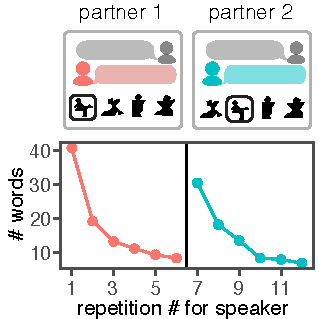
\includegraphics[scale=1.3]{./figures/clark92_compressed}
\vspace{1em}
\caption{\textit{Classic phenomena in repeated reference games.} Over multiple iterations with the same partner, speakers speakers converge on increasingly efficient referring expressions (reps.~1-6). When the listener is replaced by a new, naive partner, speakers display a key signature of partner-specificity, reverting to longer utterances before converging again with their new partner (reps.~7-12). Comprehension failures tend to be rare ($\sim 2.3\%$) throughout the experiment, indicating that speakers modulate their utterances effectively. Data from Table 3 in \protect\citeA{wilkes-gibbs_coordinating_1992}.}
\label{fig:clark92}
\end{figure}

\paragraph{P2:~Partner-specific conventions}
Because meaning is grounded in the evolving common ground shared with each partner, \emph{ad hoc} conventions established over a history of interaction with one partner are not necessarily transferred to other partners \cite{metzing_when_2003,weber_cultural_2003,brown2009partner}\footnote{We use the term ``\emph{ad hoc} convention'' \cite<inspired by>{Barsalou83_AdHocCategories} interchangeably with the more common ``conceptual pact''   \cite{BrennanClark96_ConceptualPactsConversation,IbarraTanenhaus16_FlexibilityConceptualPacts} to emphasize the theoretical relationship between this construct and the usual sense of convention referring to longer-term communal knowledge.}. 
For example, \citeA{wilkes-gibbs_coordinating_1992} paired participants for a standard repeated reference game, but after six rounds, the listener was replaced by a naive partner. 
Without partner-specific representations, we would expect speakers to continue using the short labels they had converged on with their first partner; instead, speakers reverted to the longer utterances they had initially used, and then coordinated on new \emph{ad hoc} conventions with their new partner (see Fig.~\ref{fig:clark92}).
These effects raise our second puzzle: how do community-level conventions form in the presence of such strong partner-specificity?
When are agents justified in transferring an \emph{ad hoc} convention formed with one partner to a new, unseen partner? 

One important empirical clue was provided by \citeA{fay_interactive_2010}, who examined the emergence of conventions in a lab experiment where communities of eight people played a repeated  graphical communication game similar to Pictionary, where participants produced drawings to allow their partner to identify a concept from a list of possibilities. 
The 8 participants in each network interacted dyadically with every other member of the community, in turn, for a series of seven repeated reference games. 
Strikingly, participants behaved as observed by \citeA{wilkes-gibbs_coordinating_1992} during the first few partner swaps, consistent with partner-specificity, but with subsequent partners, their initial drawings showed a gradual convergence with the  conventionalized drawings they had settled upon with previous partners, indicating a slow gradient of generalization within their community.

While intriguing, this work was limited by an extremely small sample size~($N=4$~groups)~and technical challenges facing the measurement of conventions in the graphical modality \cite<see also>{hawkins2019disentangling}.
More recent work has adopted a similar design for an artificial-language communication task \cite{raviv2019larger} but collapses across repeated dyadic interactions to exclusively analyze network-level metrics, making it difficult to assess partner-specificity.
Given these limitations of existing data, we evaluate our model's predictions using new data from a large-scale, real-time web experiment directly extending \citeA{wilkes-gibbs_coordinating_1992} to larger networks.

\paragraph{P3:~Context-sensitive conventions}

Finally, while a degree of arbitrariness is central to conventionality -- there must exist more than one solution that would work equally well -- this does not necessarily imply that all possible conventions for a given meaning are equally likely in practice, or even any convention will form at all \cite{HawkinsGoldstone16_SocialConventions}.
Indeed, functional accounts of language have frequently observed that lexical systems are well-calibrated to the needs of users under the statistics of their communicative environment \cite{gibson2019efficiency}.
This Optimal Semantic Expressivity  hypothesis \cite<OSE;>{frankblogpost} has held remarkably well for the lexical distributions found in natural languages across semantic domains like color words and kinship categories \cite{KempRegier12_KinshipCategories,regier201511,gibson2017color,kemp2018semantic}.

While such long-term, diachronic sensitivity to context has been explained by abstract principles of optimality, such as the equilibria concepts of evolutionary game theory \cite{jager2007evolution,jager2007language}, it has not yet been grounded in a cognitive and mechanistic account of the immediate, synchronic processes unfolding in the minds of individual agents while they interact.
In other words, while there is abundant empirical evidence for context-sensitivity in the \emph{outcomes} of convention formation processes, our third puzzle concerns which cognitive mechanisms  in individuals may be necessary or sufficient to give rise to such conventions \cite<see>[which raises a similar linking problem]{brochhagen2021brief}.

Repeated reference games have emerged as a promising method for probing these mechanisms in the lab. 
Such games allow researchers to  explicitly control the communicative context and observe the resulting distribution of conventions that emerge when participants communicate using artificial languages \cite{WintersKirbySmith14_LanguagesAdapt, KirbyTamarizCornishSmith15_CompressionCommunication,winters2018contextual} or natural language \cite{hawkins2020characterizing}.
While these studies are informative, it has remained challenging to directly evaluate cognitive models against the \emph{full trajectories} of convention formation on a trial-by-trial basis.
In our final section, we report new empirical data from a dyadic repeated reference task manipulating context, where simulated agents and human participants are shown exactly the same sequence of trials.

